\documentclass{article}
\usepackage[UTF8]{ctex}
\usepackage{amsmath,mathtools,geometry,pgfplots,float,mathrsfs,caption,enumerate,amssymb}
\pgfplotsset{compat=1.15}
\usetikzlibrary{arrows}
\usetikzlibrary[patterns]
\geometry{scale=0.7}

\title{第一届西西群联赛模拟一试答卷}
\author{\textit{La Campanella}}

\begin{document}
	\maketitle
	\section{填空题}
	\begin{enumerate}[1.]
		\item 39
		\item $\left(-\frac{5}{4},-1\right]$
		\item $\displaystyle 
		\begin{cases}
			\{0\},&i=j;\\
			\{\pi/3\},&|i-j|=1;\\
			\{0,2\pi/3\},&2||i-j|,|i-j|>1;\\
			\{\pi/3,\pi\},&2\nmid|i-j|,|i-j|>1.
		\end{cases}
		$
		\item $\sqrt{14}$
		\item 18
		\item $\sqrt{2}-1$
	\end{enumerate}
	\section{解答题}
	9.解: 由射影定理与正弦定理, 
	\[b=a\cos{C}+c\cos{A},\ a\sin{C}=c\sin{A}.\]
	代入原式并整理, 得
	\[\sqrt{5}\sin{A}=\cos{A}+1.\]
	等式两侧平方并利用$\sin^2{A}=1-\cos^2{A}$, 得到
	\[(\cos{A}+1)(3\cos{A}-2)=0.\]
	解得$\cos{A}=2/3.$ 由余弦定理, 得
	\[\cos{A}=\frac{b^2+c^2-a^2}{2bc}=\frac{2}{3}.\]
	即
	\[a^2=3b^2+3c^2-4bc.\]\par
	设$b/c=k\in(0,+\infty)$, 得
	\[\frac{bc}{a^2}=\frac{bc}{3b^2+3c^2-4bc}=\frac{k}{3k^2+3-4k}=\left(3k+\frac{3}{k}-4\right)^{-1}.\]
	而对于$k\in(0,+\infty)$, 有
	\[3k+\frac{3}{k}\in\left[6,+\infty\right),\]
	故
	\[\left(3k+\frac{3}{k}-4\right)^{-1}\in\left(0,\frac{1}{2}\right].\]
	11. 解: 存在. 下证明: 满足要求的点仅有$Q:(325/41,396/41)$.
	\begin{figure}[H]
		\centering
		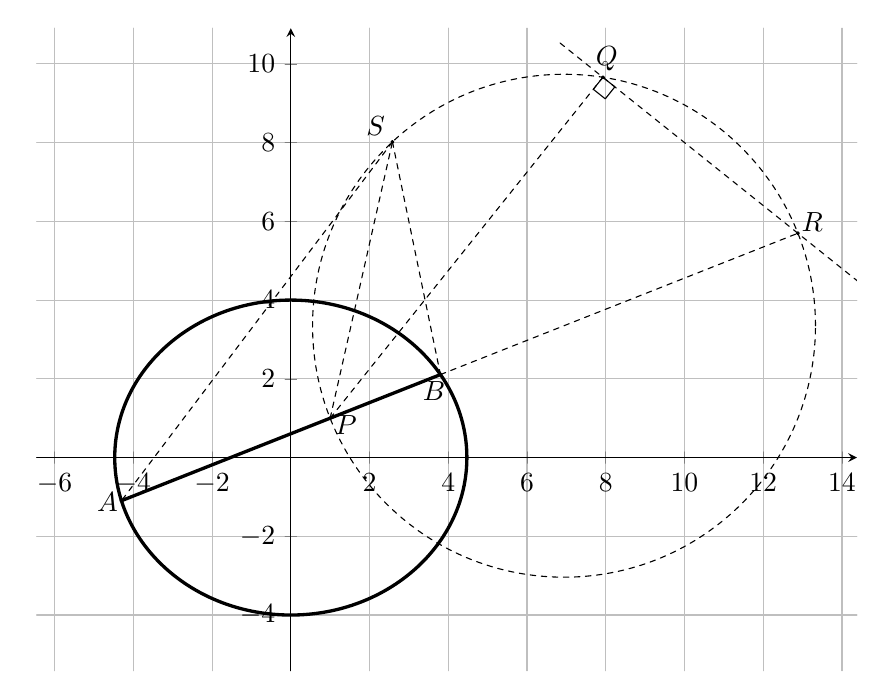
\begin{tikzpicture}[line cap=round,line join=round,>=triangle 45,x=0.5cm,y=0.5cm]
			\begin{axis}[
				x=0.5cm,y=0.5cm,
				axis lines=middle,
				ymajorgrids=true,
				xmajorgrids=true,
				xmin=-6.455230252684184,
				xmax=14.379638310264722,
				ymin=-5.414083782878573,
				ymax=10.905033532065536,
				xtick={-6.0,-4.0,...,14.0},
				ytick={-4.0,-2.0,...,10.0},]
				\clip(-6.455230252684184,-5.414083782878573) rectangle (14.379638310264722,10.905033532065536);
				\draw[line width=0.4pt] (7.683570096735823,9.35446262091978) -- (7.987644061181897,9.11120344936292) -- (8.230903232738756,9.415277413808994) -- (7.926829268292682,9.658536585365853) -- cycle; 
				\draw [rotate around={0.:(0.,0.)},line width=1.2pt] (0.,0.) ellipse (2.23606797749979cm and 2.cm);
				\draw [line width=1.2pt] (-4.3010259390493495,-1.0958743985054726)-- (3.8010819437222096,2.107467875363036);
				\draw [line width=0.4pt,dash pattern=on 2pt off 2pt] (6.939576274040141,3.348338980767882) circle (3.1934801660466947cm);
				\draw [line width=0.4pt,dash pattern=on 2pt off 2pt] (6.84109479290883,10.527124165672936)-- (16.33061964929009,2.935504280567928);
				\draw [line width=0.4pt,dash pattern=on 2pt off 2pt] (1.,1.)-- (7.926829268292682,9.658536585365853);
				\draw [line width=0.4pt,dash pattern=on 2pt off 2pt] (2.5821536022473657,8.018042391379826)-- (3.8010819437222096,2.107467875363036);
				\draw [line width=0.4pt,dash pattern=on 2pt off 2pt] (2.5821536022473657,8.018042391379826)-- (-4.3010259390493495,-1.0958743985054726);
				\draw [line width=0.4pt,dash pattern=on 2pt off 2pt] (1.,1.)-- (2.5821536022473657,8.018042391379826);
				\draw [line width=0.4pt,dash pattern=on 2pt off 2pt] (3.8010819437222096,2.107467875363036)-- (12.879152548080286,5.696677961535766);
				\begin{scriptsize}
					\draw [fill=black] (1.,1.) circle (0.5pt);
					\draw[color=black] (1.4014426503485315,0.8180200736158304) node {$P$};
					\draw [fill=black] (-4.3010259390493495,-1.0958743985054726) circle (0.5pt);
					\draw[color=black] (-4.656272438438375,-1.1277914397520838) node {$A$};
					\draw [fill=black] (3.8010819437222096,2.107467875363036) circle (0.5pt);
					\draw[color=black] (3.6409615619606606,1.6991422683484705) node {$B$};
					\draw [fill=black] (7.926829268292682,9.658536585365853) circle (0.5pt);
					\draw[color=black] (8.028215823233603,10.124873255479343) node {$Q$};
					\draw [fill=black] (12.879152548080286,5.696677961535766) circle (0.5pt);
					\draw[color=black] (13.241522142068396,5.9946129676700926) node {$R$};
					\draw [fill=black] (2.5821536022473657,8.018042391379826) circle (0.5pt);
					\draw[color=black] (2.154067858349329,8.417699003184854) node {$S$};
				\end{scriptsize}
			\end{axis}
		\end{tikzpicture}
	\end{figure}
	如图, 在直线$AB$上作点$R$, 满足
	\[\frac{AP}{PB}=\frac{AR}{RB}.\]
	设$\overrightarrow{PA}+\lambda\overrightarrow{PB}=\overrightarrow{0}$, 则有$\overrightarrow{RA}-\lambda\overrightarrow{RB}=\overrightarrow{0}$. 则
	\[\left(\overrightarrow{RP}+\overrightarrow{PA}\right)-\lambda\left(\overrightarrow{RP}+\overrightarrow{PB}\right)=\overrightarrow{0}.\]
	化简, 得
	\begin{equation}
		\overrightarrow{PR}=\frac{2\overrightarrow{AP}}{\lambda-1.}
	\end{equation}\par
	设$l_{AB}: y=k(x-1)+1$. 与椭圆方程联立, 得
	\[\left(4+5k^2\right)x^2+10k(1-k)x+5(1k)^2=0,\]
	得
	\[x_A=\frac{-5k+5 k^2-2 \sqrt{5} \sqrt{19 k^2+2 k+15}}{5 k^2+4},x_B=\frac{-5k+5 k^2+2 \sqrt{5} \sqrt{19 k^2+2 k+15}}{5 k^2+4}.\]
	则
	\[\lambda=-\frac{x_A-1}{x_B-1}=\frac{-2 \sqrt{95 k^2+10 k+75}-5 k-4}{2 \sqrt{95 k^2+10 k+75}-5 k-4}.\]
	结合(1)式, 可得
	\[x_R=x_P+\frac{2x_P-2x_A}{\lambda-1}=\frac{75+5k}{4+5k},\]
	\[y_R=k(x_R-1)+1=\frac{76k+4}{4+5k}.\]
	不难发现
	\[4x_R+5y_R=80.\]
	即$R$的轨迹为$4x+5y=80$.\par
	作以$PR$为直径的圆, 并设在$l_{AB}$转动时所有这样的圆的集合为$K$. 则由阿氏圆, 此圆即为所有满足$\angle ASP=\angle BSP$的$S$的轨迹. 故满足题目的$Q$应当在$K$中的每一个圆上.\par
	设$R$在直线$4x+5y=80$上的投影为$Q'$, 则$K$中的每个圆均经过$Q'$. 同时每个圆经过$P$, 而两个圆不可能有三个交点, 故至多存在两个点, 使$K$中每个圆均经过此两点. 故这样的$Q$是唯一的.\par 
	不难算出$P$在$4x+5y=80$的投影为$Q:(325/41,396/41)$.
\end{document}
